% !TEX root = D:\Users\Ignacio\Documentos\Escuela\CC3002 - Metodologías de Diseño y Programación\apunte-y-ejercicios\src\latex\Apunte.tex
\subsection{Configuración de un proyecto}
  Por defecto, al crear un proyecto se crean varias carpetas y archivos en el directorio que hayamos
  especificado, pueden ver esto en la pestaña \texttt{Project} ubicada a la izquierda del 
  \textit{IDE} (figura \ref{fig:project-fs}), la única carpeta que nos interesará es \texttt{src} 
  que es donde guardaremos todo nuestro código.

  \begin{figure}[ht!]
    \centering
    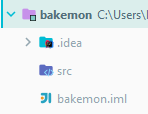
\includegraphics{img/Profundizando en Java/IntellJ Project FS.png}
    \caption{Organización inicial de un proyecto}
    \label{fig:project-fs}
  \end{figure}

  Con el proyecto ya creado puede que sea necesario revisar las configuraciones (en la mayoría de 
  los casos la configuración por defecto de \textit{IntelliJ} debiera ser suficiente, pero es bueno
  conocer este menú).
  Para ir a las configuraciones del proyecto accedan mediante el menú principal en \texttt{File | 
  Project Structure}.

  Este menú tiene varias pestañas, pero nos enfocaremos en 2.

  Comencemos por la pestaña \texttt{Project Settings | Project}, aquí podrán encontrar 4 opciones a 
  configurar (vean la figura \ref{fig:ij-project-settings}).
  El primer campo es el nombre del proyecto (por si quisiéramos cambiarle de nombre en algún 
  momento). 
  El segundo es el \textit{SDK} que indica la versión del \textit{JDK} que vamos a 
  utilizar.
  La opción siguiente es para decirle al \textit{IDE} las funcionalidades de qué 
  \textit{SDK} utilizar, en general esto va a ser igual que la opción anterior, pero sirve para 
  escribir código compatible con \textit{SDKs} más antiguos (e.g. trabajamos en un proyecto con otra
  persona que tiene instalado \textit{Java 9} pero nosotros tenemos \textit{Java 11}, en este caso 
  conviene fijar este campo como \textit{Java 9}).
  Por último tenemos \texttt{Project compiler output}, aquí es donde se almacenaran los archivos 
  generados por el compilador, este directorio \textbf{debe} existir (la convención es tener una 
  carpeta \texttt{out} en la raíz del proyecto, en nuestro caso sería \texttt{.../Pokemon/out}).

  \begin{figure}[ht!]
    \centering
    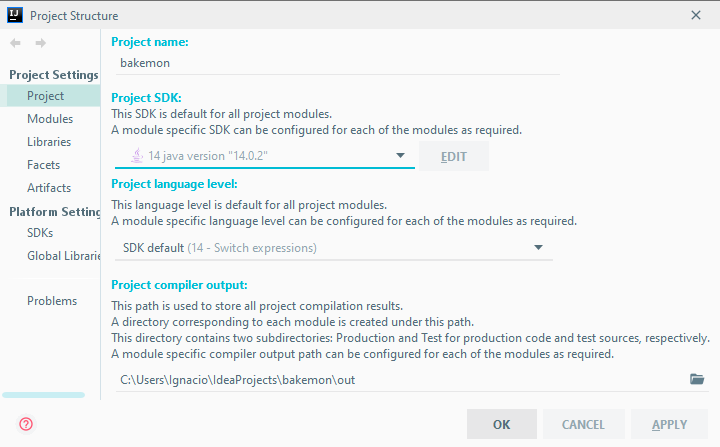
\includegraphics[width=0.7\textwidth]{img/Profundizando en Java/IntelliJ Project Settings.png}
    \caption{Configuraciones del proyecto}
    \label{fig:ij-project-settings}
  \end{figure}

  La siguiente pestaña es \texttt{Project Settings | Modules}, aquí podemos ver la estructura de los
  directorios del proyecto.
  Es importante que la carpeta \texttt{src} esté marcada como \texttt{Sources} para que el 
  \textit{IDE} sepa que ahí es donde se ubica el código de la aplicación (tomen como ejemplo la 
  figura \ref{fig:ij-modules}).

  \begin{figure}[ht!]
    \centering
    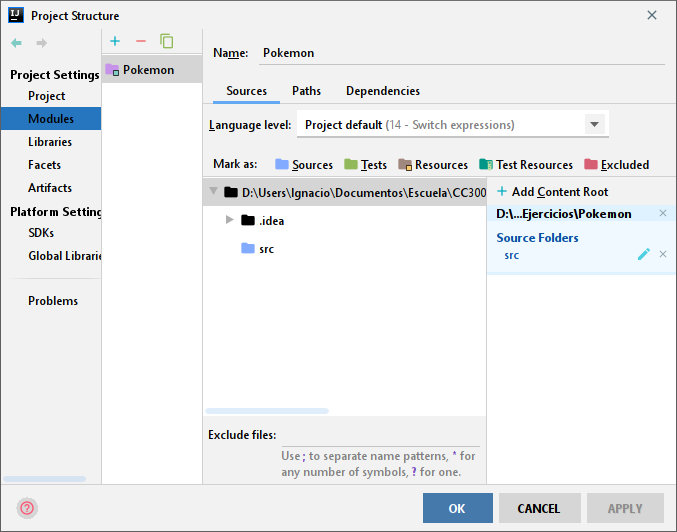
\includegraphics[width=0.7\textwidth]{img/Profundizando en Java/IntelliJ Project Modules.png}
    \caption{Estructura de directorios del proyecto}
    \label{fig:ij-modules}
  \end{figure}

  El resto de las pestañas también son importantes,\footnote{!`Todas las pestañas son válidas!} y 
  veremos algunas de estas más adelante en el apunte.
%